% Өгөгдлийн сангийн ER диаграмм — standalone TikZ
% Compile: xelatex er_diagram.tex
\documentclass[border=10pt]{standalone}
\usepackage{fontspec}
\setmainfont{Times New Roman}
\usepackage{tikz}
\usetikzlibrary{arrows.meta, positioning, calc, shapes.multipart}

\begin{document}

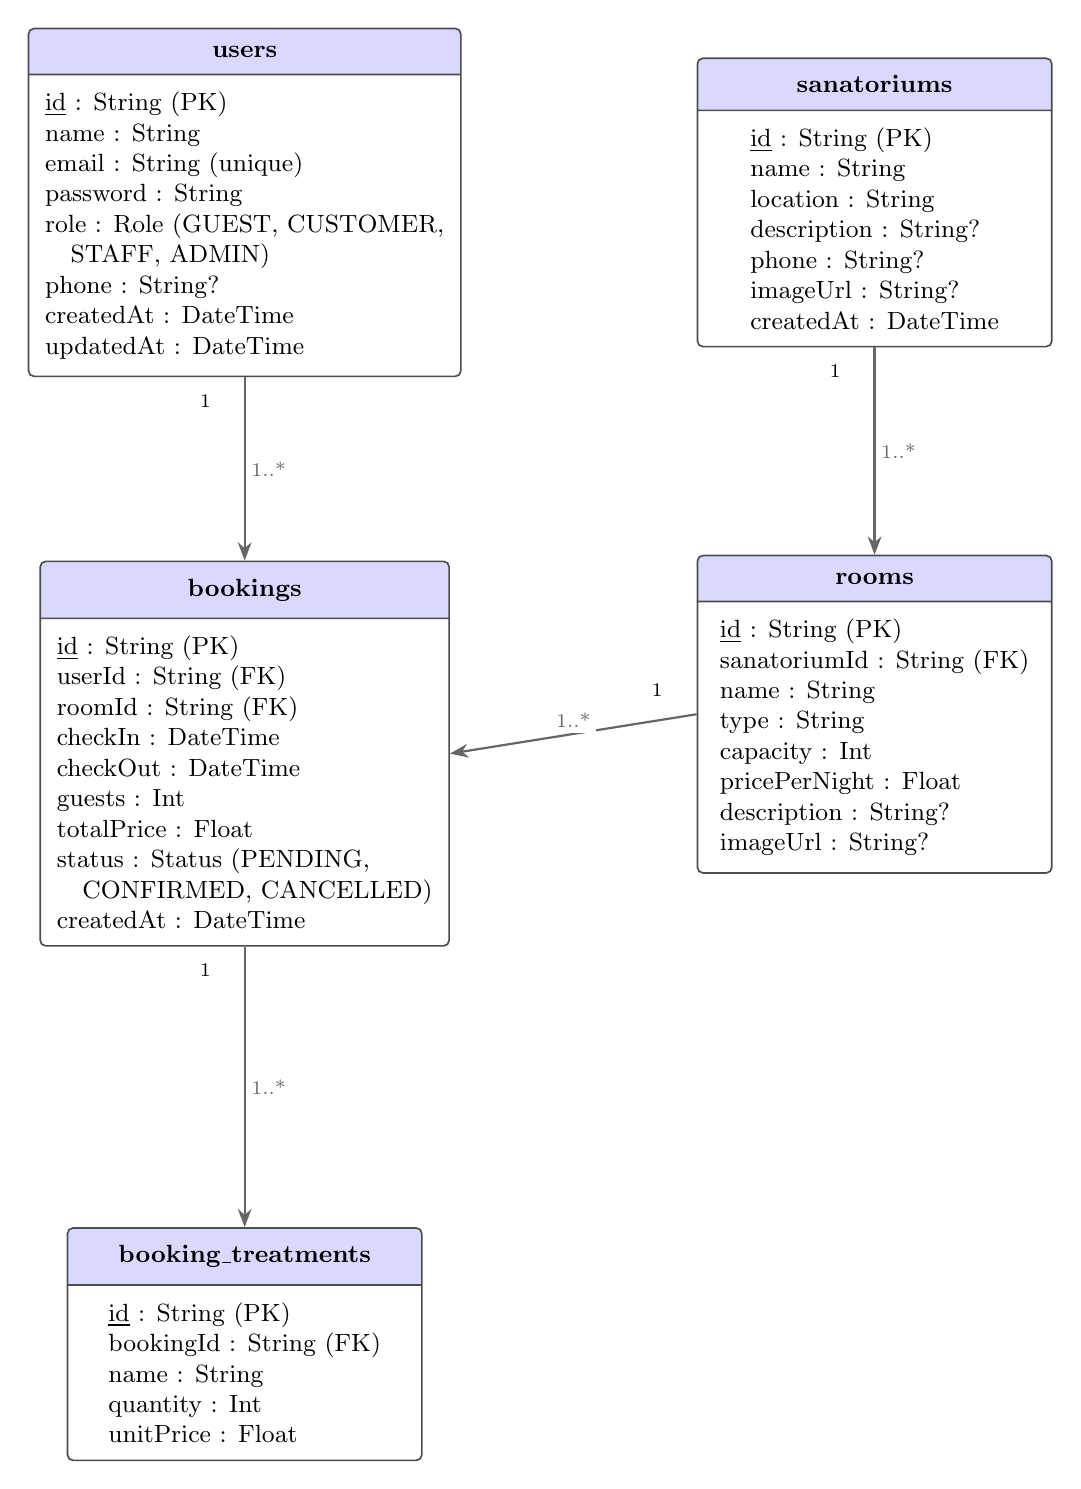
\begin{tikzpicture}[
  % ---- styles ----
  entity/.style = {
    rectangle split, rectangle split parts=2,
    rectangle split part fill={blue!15, white},
    draw=black!70, line width=0.6pt,
    rounded corners=2pt,
    minimum width=4.5cm,
    font=\small,
    align=left,
    inner sep=6pt
  },
  entitytitle/.style = {font=\small\bfseries},
  rel/.style = {-Stealth, thick, black!60},
  rellabel/.style = {font=\scriptsize, fill=white, inner sep=2pt}
]

% ============ ENTITIES ============

% --- users ---
\node[entity] (users) at (0, 0) {
  \textbf{users}
  \nodepart{second}
  \underline{id} : String (PK)\\
  name : String\\
  email : String (unique)\\
  password : String\\
  role : Role (GUEST, CUSTOMER,\\
  \quad STAFF, ADMIN)\\
  phone : String?\\
  createdAt : DateTime\\
  updatedAt : DateTime
};

% --- sanatoriums ---
\node[entity] (sanatoriums) at (8, 0) {
  \textbf{sanatoriums}
  \nodepart{second}
  \underline{id} : String (PK)\\
  name : String\\
  location : String\\
  description : String?\\
  phone : String?\\
  imageUrl : String?\\
  createdAt : DateTime
};

% --- rooms ---
\node[entity] (rooms) at (8, -6.5) {
  \textbf{rooms}
  \nodepart{second}
  \underline{id} : String (PK)\\
  sanatoriumId : String (FK)\\
  name : String\\
  type : String\\
  capacity : Int\\
  pricePerNight : Float\\
  description : String?\\
  imageUrl : String?
};

% --- bookings ---
\node[entity] (bookings) at (0, -7) {
  \textbf{bookings}
  \nodepart{second}
  \underline{id} : String (PK)\\
  userId : String (FK)\\
  roomId : String (FK)\\
  checkIn : DateTime\\
  checkOut : DateTime\\
  guests : Int\\
  totalPrice : Float\\
  status : Status (PENDING,\\
  \quad CONFIRMED, CANCELLED)\\
  createdAt : DateTime
};

% --- booking_treatments ---
\node[entity] (treatments) at (0, -14.5) {
  \textbf{booking\_treatments}
  \nodepart{second}
  \underline{id} : String (PK)\\
  bookingId : String (FK)\\
  name : String\\
  quantity : Int\\
  unitPrice : Float
};

% ============ RELATIONSHIPS ============

% users 1──* bookings
\draw[rel] (users.south) -- node[rellabel, right, pos=0.5] {1..*} (bookings.north);
\node[rellabel] at ($(users.south) + (-0.5, -0.3)$) {1};

% sanatoriums 1──* rooms
\draw[rel] (sanatoriums.south) -- node[rellabel, right, pos=0.5] {1..*} (rooms.north);
\node[rellabel] at ($(sanatoriums.south) + (-0.5, -0.3)$) {1};

% rooms 1──* bookings
\draw[rel] (rooms.west) -- node[rellabel, above, pos=0.5] {1..*} (bookings.east);
\node[rellabel] at ($(rooms.west) + (-0.5, 0.3)$) {1};

% bookings 1──* treatments
\draw[rel] (bookings.south) -- node[rellabel, right, pos=0.5] {1..*} (treatments.north);
\node[rellabel] at ($(bookings.south) + (-0.5, -0.3)$) {1};

\end{tikzpicture}
\end{document}
